% REPORT.TEX - University of Warwick Reports / Dissertations / Projects
% 
% Author - Chris Quinn 28/06/2020
% 
%
% A template for students and masters dissertations, flexible for your
% needs.
%
% This is the main .tex which will tell the compiler to include everything, 
% each chapter/section is then in folders for convenience, as you include more 
% images it can get harder and harder to manage.
%
% First things first, declaration of the document class along with the packages % we need.
%
% P.S. Sorry about the back to the future references, I used them to show some 
% example work possible




\documentclass[pdftex,10pt,a4paper,oneside]{article}
%Can change the pt, papersize etc.

\usepackage{amsmath} %For both in-line and equation mode
\numberwithin{equation}{section} %Numbering of our equations per section
\usepackage{algorithm}
\usepackage{algorithmic} %Algorithm styles, need to be nested for the example shown
\usepackage{fancyhdr} %For our headers
\usepackage{graphicx} %Inserting images
\usepackage{lipsum}  %Blank text fill, delete me when finished
\usepackage{setspace} %Spacing on the front page for crest and titles
\usepackage[]{fncychap} % Styles can be Sonny, Lenny, Glenn, Conny, Rejne, Bjarne and Bjornstrup
\usepackage[hyphens]{url} %Deals with hyphens in urls to make them clickable
\usepackage{xcolor} %Great if you want coloured text
\usepackage{tabularx}
\usepackage{appendix} %Take a wild guess slick



%KEEP THIS ONE LAST it's quite buggy, it allows you to click on links within the pdf and web links without changing the colour. The mouse cursor simply changes its icon to indicate to the user. Great tool - still awkward
\usepackage[hidelinks]{hyperref}



%This will tell the compiler to do the header style, page and spacing between the header and text
\fancyhf{}
\pagestyle{fancy}
\renewcommand{\headrulewidth}{0.2pt}


%%%%%%%%%%%%%%%%%%%%%%%%%% DOCUMENT STARTS %%%%%%%%%%%%%%%%%%%%%%%%%%%%%



%Lets begin the document, some chapters have examples in to give you an idea 
\begin{document}

% !TEX root =  ../Report.tex

\thispagestyle{empty}

\begin{spacing}{2}
	\begin{center}
		
\includegraphics[scale = 0.45]{Preamble/WarwickCrest.pdf}
		%Two images here for University of Warwick students, the colour crest and the black and white crest. Replace as appropriate!
	\end{center}
	\vspace{5mm}
	\begin{center}
		\textbf{\begin{LARGE}
		A Template for computer science projects
		\end{LARGE}}
		\vspace{5mm}
	\end{center}
	\begin{center}
		{\large CS101 Flux Capacitors and their Applications}\\
		\vspace{20mm}
	\end{center}
	\begin{center}
		\textbf{\large Marty McFly}
		\vspace{20mm}
	\end{center}
	\begin{center}
	     {\large Supervisor: Dr. Emmett Brown }\\
		\textbf{\large Department of Computer Science}\\
		{\large University of Hill Valley}\\
		{\large 1955-1985\\}
	\end{center}
\end{spacing}

\pagenumbering{roman}



\section*{Abstract}
\addcontentsline{toc}{section}{Abstract}
\vspace{2cm}

\large
When this thing gets up to 88 mph, you're gonna see some serious s$\cdot \cdot \cdot$.\\

\vspace{1cm}

\noindent \textit{Keywords: Flux Capacitor, 1.21 Gigawatts, Calvin Klein}
\section*{Acknowledgements}
\addcontentsline{toc}{section}{Acknowledgements}

\vspace{2cm}

\large

Always good to acknowledge people. %(yes, there are definitely people to acknowledge )
%Comment the whole thing out if you don't want it

\section*{Abbreviations}
\addcontentsline{toc}{section}{Abbreviations}
\large 
Flux Capacitor \hfill FC\\
Gigawatt \hfill GW\\



\tableofcontents

% Once you start inserting figures, tables and algorithms then they % will start appearing here in the lists. 
%
% The captions and names you give them will appear here. The 
% numbering can either be:
%
%     Natural (1,2,3,...) 
%     Sectional (1.1, 1.2 for chapter 1. 2.1, 2.2,... for chapter 2) 



\listoffigures
\addcontentsline{toc}{section}{List of Figures}
\numberwithin{figure}{section}

\listoftables
\addcontentsline{toc}{section}{List of Tables}
\numberwithin{table}{section}

%Delete me if you're not putting algorithms in or you don't want it as contents. Same applies with the two above ^
\listofalgorithms
\addcontentsline{toc}{section}{List of Algorithms}
\numberwithin{algorithm}{section}

\newpage


\pagenumbering{arabic}

\lfoot{\centering \thepage}



% !TEX root =  ../Report.tex

\section{Introduction}
\label{sec:Introduction} 
%To make a call to the introduction, put \ref{sec:Introduction}. Overleaf can auto-fill it for you

\lipsum[1]
% !TEX root =  ../Report.tex
\section{Figures, tables, algorithms}
\label{sec: figs tables algos}

The researcher and the supervisor both attended a photography for the new hill valley clock tower. This can be seen in figure \ref{fig:clock tower photo}.

\begin{figure}[h!]
    \centering
    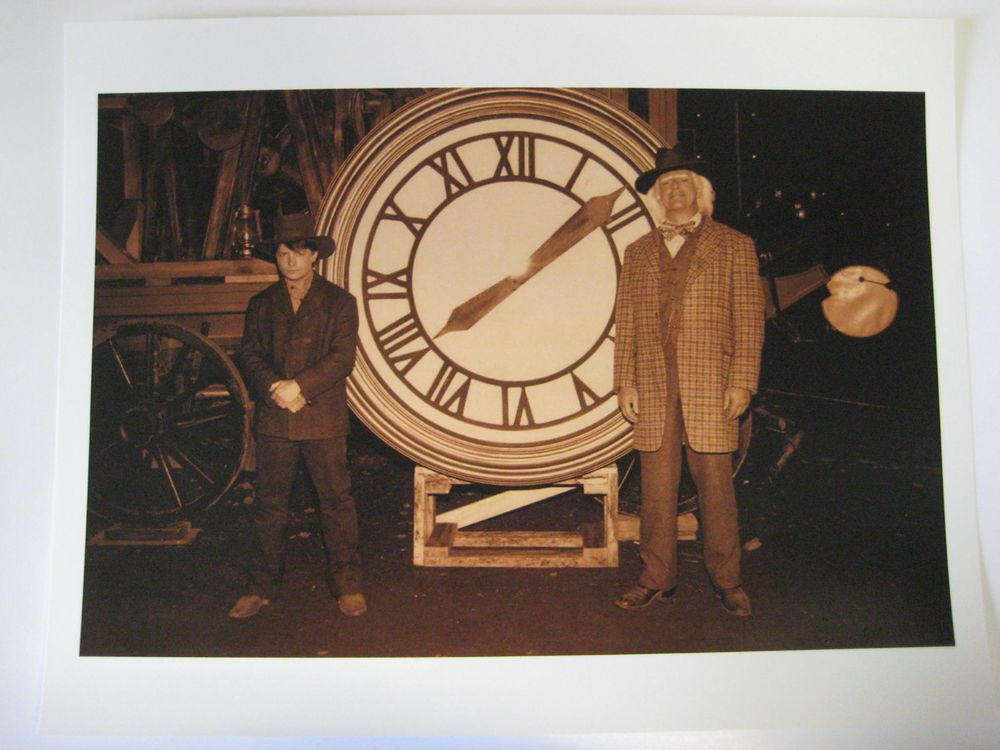
\includegraphics[width=\textwidth]{Report/Chapter2/doc_and_marty.jpg}
    \caption{The Researcher and Supervisor}
    \label{fig:clock tower photo}
\end{figure}

\noindent Again from figure \ref{fig:clock tower photo} we can see the researcher on the \textit{left} and the supervisor on the \textit{right}.\\

From this, a table was made for some of the items needed for temporal experiment number one to undergo completion. This is set to occur on \texttt{October 26, 1985, 1:18 A.M}.

\begin{table}[H] 
\begin{tabularx}{\textwidth}{| X | X |}
    \hline
     Item & Description  \\ \hline
     2 x Pocket Clocks & For measurement in time difference of machine and present time \\ \hline
     Einstein & The Dog test pilot \\ \hline
     JVC GR-C1 & VHS Camcorder \\ \hline
\end{tabularx}
\caption{Inventory list for temporal experiment number one}
\label{table: inventory}
\end{table}

%!TEX root =  ../Report.tex

\section{Chapter 3}                               
\label{sec: Chapter 3}

\lipsum[3]


%Rename me as appropriate
% !TEX root =  ../Report.tex

\section{Chapter 4}
\label{sec: Chapter 4}
\lipsum[4]
%Here are some subsections so that they will appear on the contents

\subsection{Sub Chapter}
\label{sec: sub chapter in chapter 4}
\lipsum[5]



% !TEX root =  ../Report.tex

\section{Chapter 5}
\label{sec: Chapter 5}

\lipsum[6]

% !TEX root =  ../Report.tex

\section{Chapter 6}
\label{sec: Chapter 6}

\lipsum[7]
% !TEX root =  ../Report.tex

\section{Chapter 7}
\label{Sec: Chapter 7}

\lipsum[8]


%!TEX root =  ../Report.tex

\section{Chapter 8}
\label{sec:Chapter 8}

\lipsum[9]



% !TEX root =  ../Report.tex
\section{Making a reference}
\label{sec: Reference}

\noindent In this chapter we shall do a reference to an entry in the bibliography, \texttt{bibliography.bib}. \\

What we know of the invention of the flux capacitor is that Dr. Emmett Brown thought of this when hanging a clock in the bathroom. He was standing on his porcelain sink and slipped because it was wet, the resulting hit on the head was apparently a cause to this invention \cite{example}.\\

The corresponding sketch made on this day has been attached in appendix \ref{appx: Flux Sketch}.


%Keep adding folders as to your desires

\bibliographystyle{abbrv}
\bibliography{bibliography}

\begin{appendices}
\addcontentsline{toc}{section}{Appendices}


\section{The Flux Sketch}
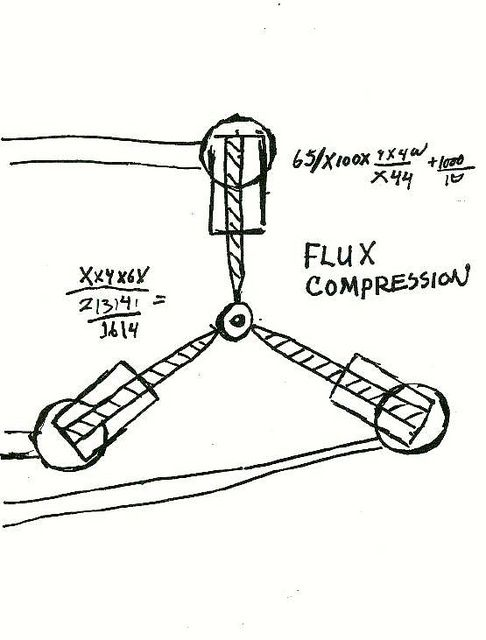
\includegraphics[width=\textwidth]{Report/Appendices/flux_sketch.jpg}
\label{appx: Flux Sketch}



\end{appendices}


\end{document}
